\chapter{Encoding of Orientation Variance through Recurrence in V1}

\begin{flushright}
    \textit{''Representations, at a minimum,\\
    must potentially be able to stand in for the things they represent.''}\\
    Chris Eliasmith, How to Build a Brain, 2013
\end{flushright}

\chaptertoc{}



\section{Introduction: Orientation Selectivity in V1}
\subsection{Orientation Selectivity and Representations in the (Visual) Cortex}
As we've largely emphasized so far, orientation selectivity is a hallmark feature of the primary visual cortex. As the first functional element of the visual hierarchy, oriented receptive field form the basis of our understanding of visual processing in the cortex. This is a stereotypical role for a primary sensory cortex, which often exhibit a well-defined invariant feature code (see chapter 3) based on the sensory space they represent~\cite{carandini2012normalization, keller2018predictive}, and acting as the foundation for the downstream computations. For example, the elementary units of voices is neural encoding of tonality and frequency-defined signals~\cite{belin2011understanding}, that of bodily parts is spatially defined segments~\cite{camon2019timing}, and that of vision is our edges of interest, in this manuscript. Examining such foundational elements of image descriptors is a longstanding tradition in the field of visual neuroscience, especially within the framework of hierarchical networks~\cite{van1992information}.

\begin{figure}[h!t]
\vspace{0.1cm}
\centering
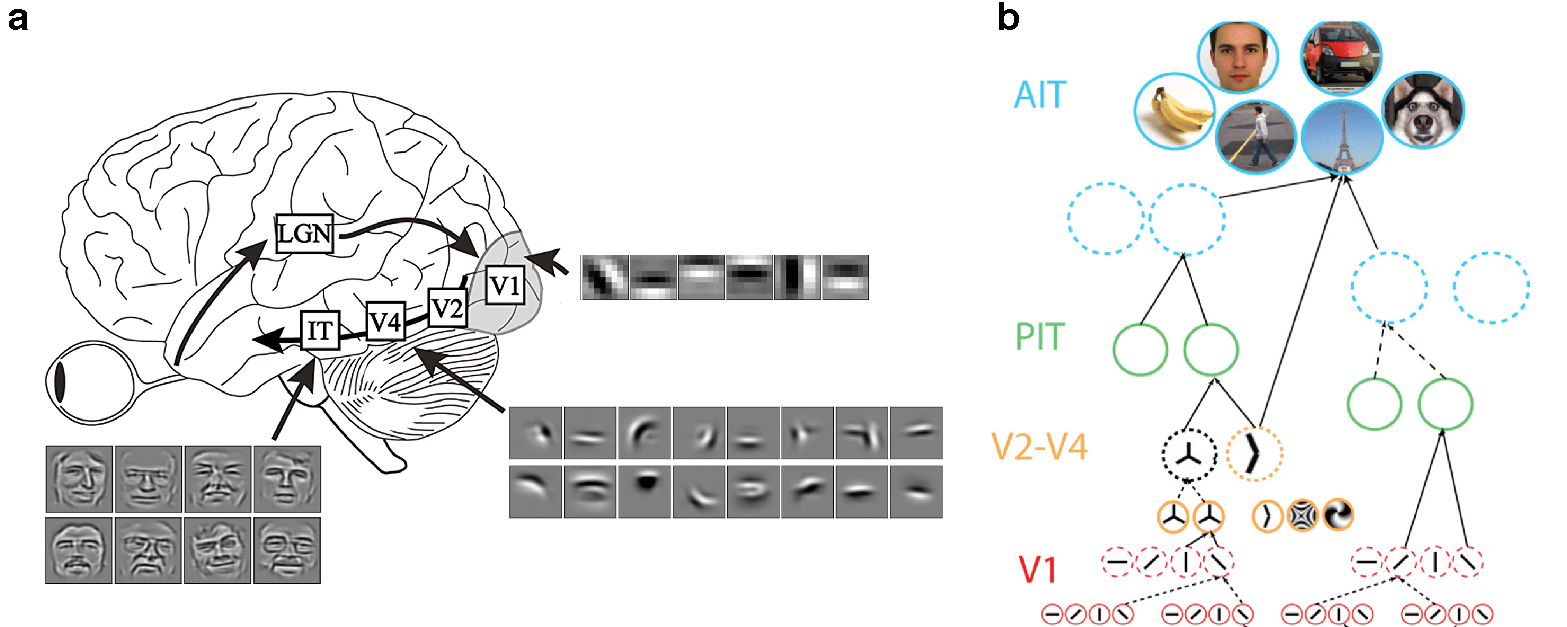
\includegraphics[width=1.\textwidth]{fig/chap4_hierarchical.pdf}
\caption[Hierarchical model of the visual cortex.]{Hierarchical model of the visual cortex (a), oftenmost reflected in the current view of computer vision models (b). Adapted from~\cite{serre2010neuromorphic}.}
\label{fig_chap4_hierarchical}
\end{figure}

In \gls{V1}, the basis of the neural code is a visual one, and has thus the advantage of being easily conceptualized and visualized. This ease-of-understanding of \gls{V1} receptive field, supported by six decades of rich literature, makes orientation selectivity a focal point in of numerous PhD theses, serving either as a principal subject of study or, as is the case here, as an angle of attack to explore theoretical frameworks with testable hypotheses. Most often, this serves to study visual processing as a feedforward model~\cite{kreiman2020beyond}, positing a sequential series of computations wherein basic visual components like edges are integrated to form progressively complex representations such as angles, textures, and eventually high-level objects, as observed in different visual cortical areas (V1, V2, V4, IT)~\cite{lamme1998feedforward}. The feedforward model proposes a structured pathway through which visual information is processed and refined at each subsequent level, contributing to a global, coherent perception of the visual world, as shown in Figure~\ref{fig_chap4_hierarchical}. For the sake of argumentation of this thesis, this view can be advantageous. Hierarchical modelling requires that separate features will be processed in separate areas, and as such, separate feature variances to be also localized and confined within each cortical area.

A notable limitation of the feedforward model lies in its inability to effectively distinguish between perceptions driven by bottom-up sensory input and the self-generated sensory feedback resulting from an organism's actions~\cite{von1950reafferenzprinzip,keller2018predictive}. In the case of vision, the visual flow stemming from eye movements could trigger an optokinetic reflex, akin to the reflexive response which stabilizes our view as we are reading this manuscript. Should an organism fail to discern between external and self-generated inputs, this reflex would inhibit any eye movement. As such, it follows logically that visual processes must also contain some form of feedback.
A simplistic strategy to mitigate this issue could be simply cancelling the predictable consequences of self-generated sensory feedback, by sending an efference copy of a motor command. 
Conceptually, such transformative processes require an internal model, can be viewed as equivalents to a simulation of the external world and its consequences for the organism. In a rather simple way (Figure~\ref{fig_chap4_representational_framework}), this extends the general feedforward representation framework into a predictive one, as used in this thesis~\cite{friston2016active}.

\begin{figure}[h!tbp]
\vspace{0.1cm}
\centering
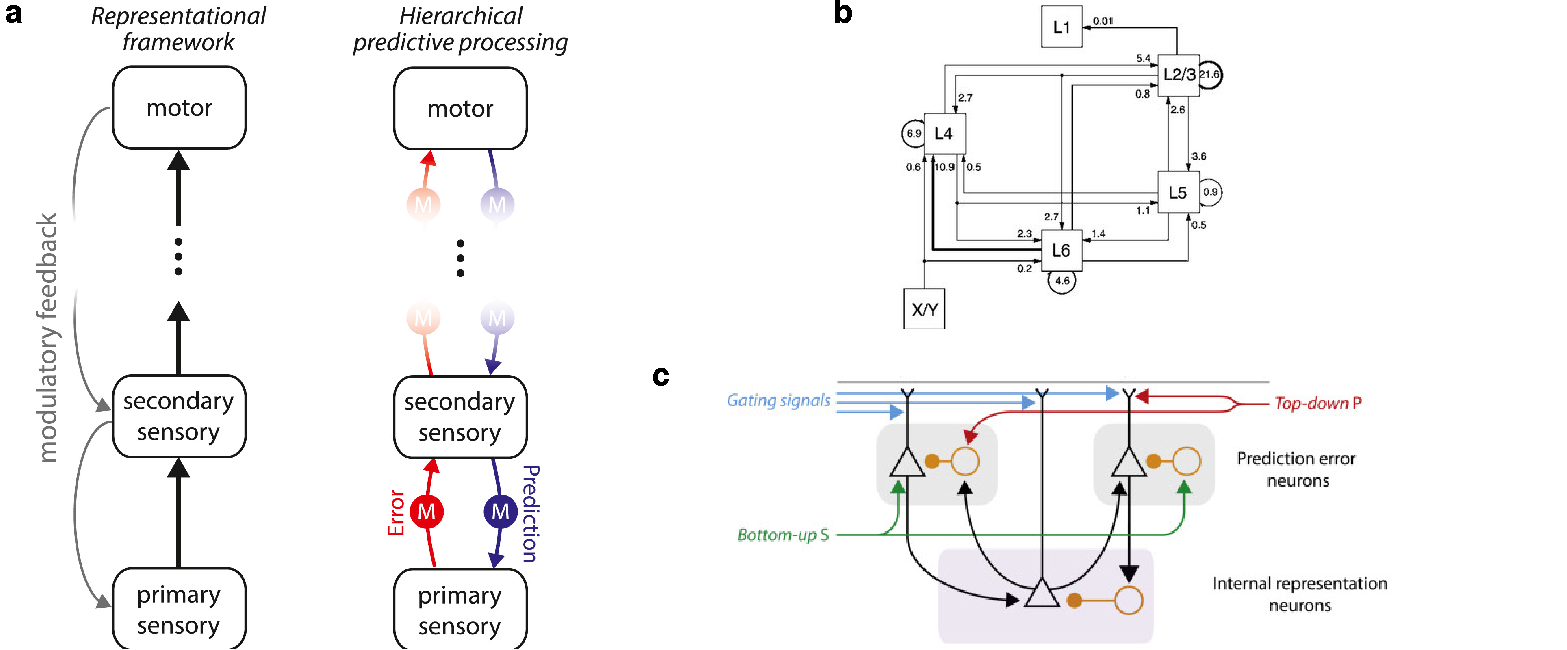
\includegraphics[width=1.\textwidth]{fig/chap4_representational_framework.pdf}
\caption[Representational and predictive frameworks.]{Representation and predictive frameworks in neuroscience. (a) Predictive coding extends the classical representational framework with the addition of prediction and related error neural elements. At the relevant level of scale here, this extends the canonical microcircuit~\cite{douglas1989canonical} (b) into a predictive neural circuit (c). Adapted from \cite{douglas1989canonical} and~\cite{keller2018predictive}.}
\label{fig_chap4_representational_framework}
\end{figure}

Although this doesn't challenge the notion that orientation selectivity is an optimal feature for a model of vision, it does offer an alternative perspective for the present chapter. Our aim here is to illustrate that, within a predictive modelling framework, \gls{V1} neurons don't just represent a singular feature, but also its variance, encoding a probabilistic distribution that form parts of a generative model.



\subsection{The Origin of Orientation Selectivity in the Cortex}
Pinpointing the origin of an invariant representation of images implemented within a biological neural network is a non-linear and non-trivial task. As such, there are as many theories related to "how" orientation selectivity emerges as there are theories as to "why" it exists. While it is impossible to make an exhaustive list of all phenomenological accounts and their myriad of variations, they can be grouped in three aspects:
\begin{itemize}
    \item Orientation selectivity emerges through converging, feedforward interactions.
    \item Orientation selectivity is refined by local (i.e. within a cortical area) recurrent, horizontal interactions.
    \item Orientation selectivity is modulated by extrastriate feedback interactions. 
\end{itemize}
As is the case with many complex biological questions framed as multiple choice, the answer is "all of the above, mixed non-linearly" (Figure~\ref{fig_chap4_vidyasagar}).

\begin{figure}[h!tbp]
\vspace{0.1cm}
\centering
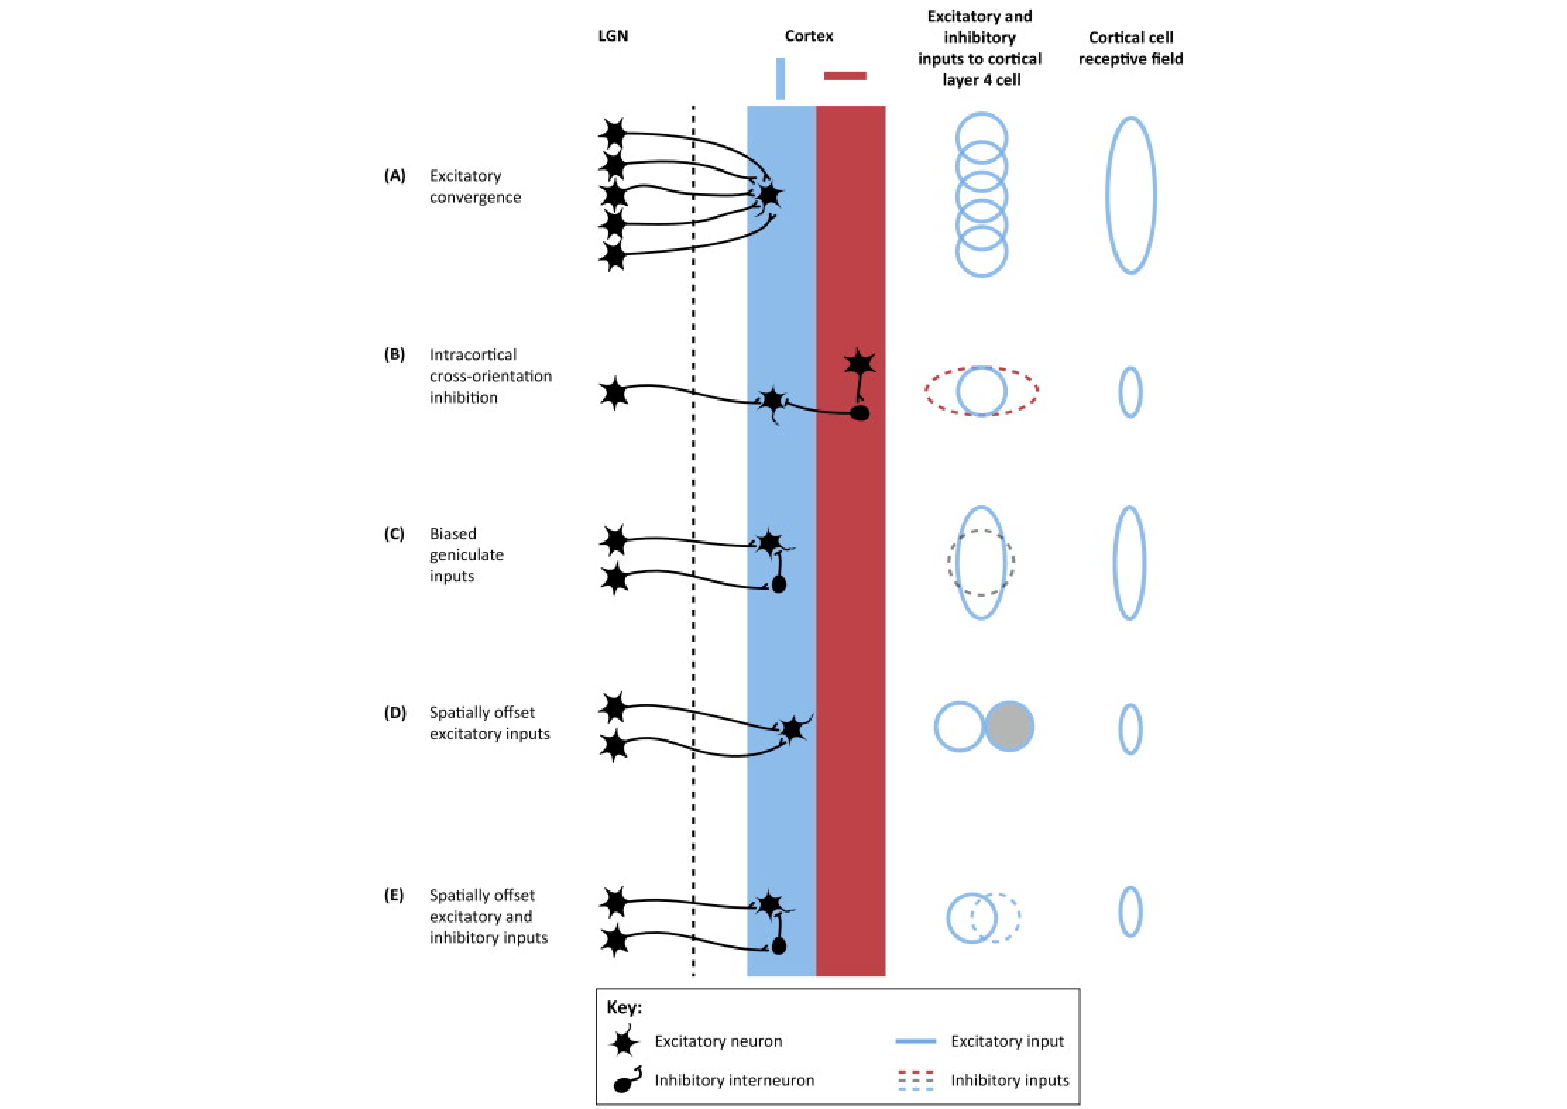
\includegraphics[width=.8\textwidth]{fig/chap4_vidyasagar.pdf}
\caption[Possible mechanisms for orientation selectivity.]{Possible mechanisms accounting for the existence of orientation selectivity, reproduced from~\cite{vidyasagar2015origins}.}
\label{fig_chap4_vidyasagar}
\end{figure}

The feedforward explanation for the emergence of orientation selectivity aligns intuitively with the feedforward representational framework discussed earlier. This "canonical" model, as introduced by Hubel and Wiesel in their seminal work~\cite{hubel1962receptive}, frames orientation selectivity as arising from the convergence of isotropic receptive fields from the \gls{LGN} to \gls{V1}. While this has been validated experimentally several times~\cite{ferster1986orientation, chapman1991relation}, such studies fail to explain the presence of (minor) orientation tuning before \gls{V1}. Specifically, when cortical networks are silenced to exclusively observe \gls{LGN} input to \gls{V1}, the resulting input is already sharply orientation-tuned~\cite{ferster1996orientation}. 
This could stem from the fact that some \gls{LGN} cells are already slightly tuned to orientation, perhaps through a certain degree of retino-\gls{LGN} convergence~\cite{xu2002primate,tan2011orientation,van2013transformation}. Indeed, even with a single thalamic oriented neuron, it is possible to obtain an excitatory orientation-tuned response in a connected \gls{V1} neuron~\cite{kara2002spatial}. 

\begin{figure}[h!tbp]
\vspace{0.1cm}
\centering
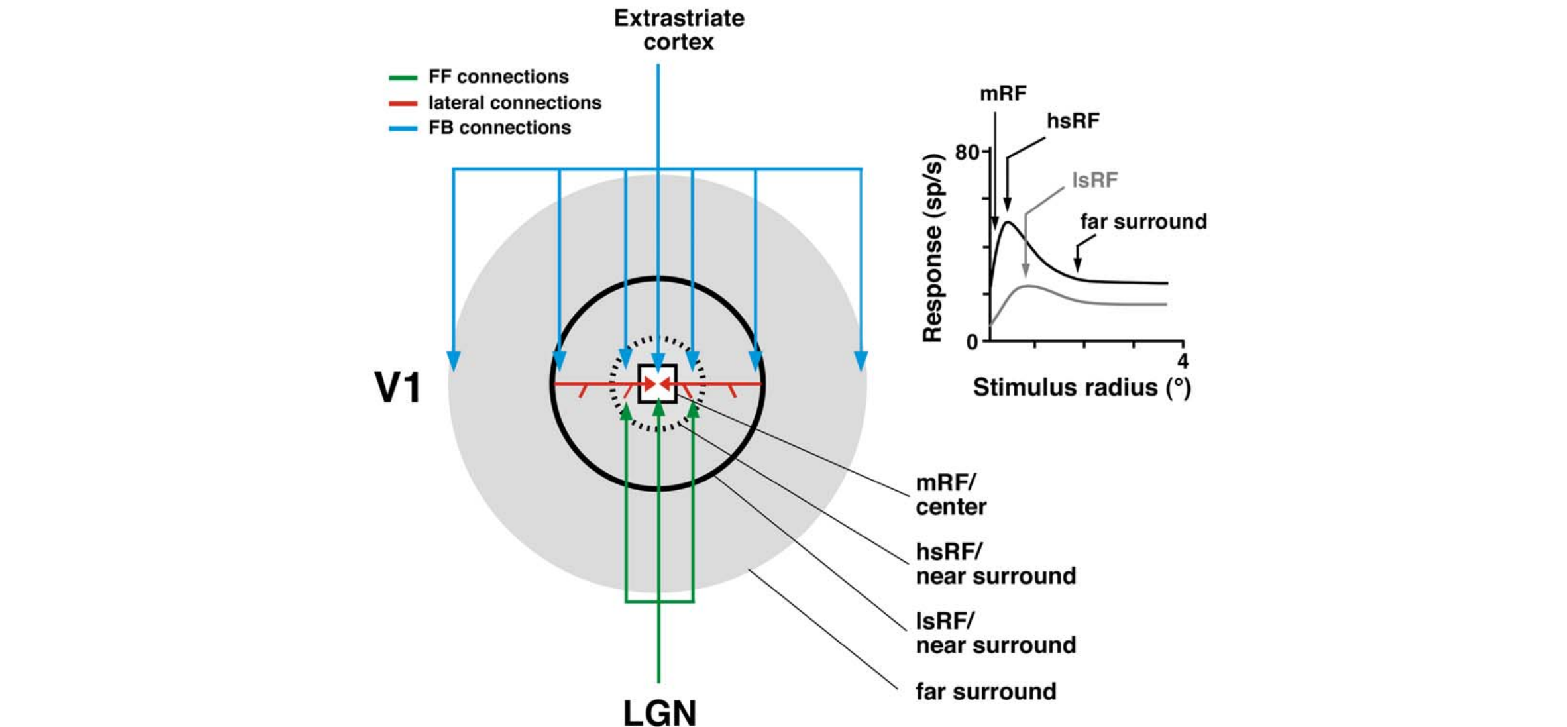
\includegraphics[width=1.\textwidth]{fig/chap4_angelucci.pdf}
\caption[Spatial extent of \gls{V1} connections.]{Spatial extent and response induced by feedforward (FF), lateral and feedback (FB) connections. Adapted from~\cite{angelucci2006contribution}.}
\label{fig_chap4_angelucci}
\end{figure}

This feedforward account of orientation selectivity is typically contrasted to the intracortical recurrent hypothesis. At the meso-scale of \gls{V1}, orientation selectivity is arranged in a "map", where neighboring neurons have heterogeneous preference~\cite{grinvald1986functional}. Long-range horizontal axons have been reported to preferentially bind to distant columns of similar orientation preferences in the cat \gls{V1}, with short-range recurrent connectivity being more heterogeneous~\cite{chavane2011lateral, chavane2022revisiting}. This would allow having interactions between neurons tuned to different orientation at short range, as we will put forward in the present article, whilst maintaining the possibility to prime contours made of similar orientation at long range. Cross-orientation inhibition within the cortex can theoretically perform orientation sharpening~\cite{priebe2012mechanisms}. This could either be responsible, on its own, for generating orientation selectivity~\cite{hansel2012mechanism}, or could serve to refine the feature emerging from the feedforward convergence. Additional mechanisms encompass voltage-sensitive mechanisms with precise location within the dendritic tree, but also intracortical excitation emanating from cells that are tuned to analogous orientations ~\cite{vidyasagar1996multiple, priebe2012mechanisms,vidyasagar2015origins}.

This also yields an interesting counter-observation, given that precisely organized orientation maps are solely present in \gls{V1} of carnivora and primates~\cite{jang2020retino}. Rodent, on the other end, have a "salt-and-pepper" (random) topology of orientation detectors, with no specific spatial mapping onto the cortex. However, through a delicate balance of excitation and inhibition, it is also possible that these networks recurrently create orientation selective neural activity~\cite{hansel2012mechanism}. This is corroborated by the notion that recurrent interactions among potentially isotropic cortical neurons can yield properties akin to those arising from feedforward interactions. In other terms, this implies that functional convergence, whether feedforward or recurrent, is an inherently viable mechanism for the emergence of orientation selectivity. Extending this idea, one can also think of the complex cells (see Introduction 2.1.1.2.) as either a convergence of simple cells, but also as recurrently "amplified" simple cells~\cite{chance1999complex}.



Given that these rodents also exhibit orientation tuning within the \gls{LGN}~\cite{tan2011orientation}, this raises additional questions. Do these phenomena reflect unique characteristics specific to certain species, or do they suggest a more comprehensive need to re-evaluate established beliefs about orientation selectivity? This question becomes especially pertinent when we consider the wide range of species exhibiting pronounced orientation tuning within the cortex. This possible difference in strategy for orientation selectivity might also speak of different strategies for processing associated variance, between primates, cats and mice. As we shall see at the end of this chapter, primates and cats seemingly exhibit similar behavior, but recordings on mice are currently underway in our laboratory, and will be discussed in the Conclusion of this thesis. 

\begin{figure}[htbp]
\vspace{0.1cm}
\centering
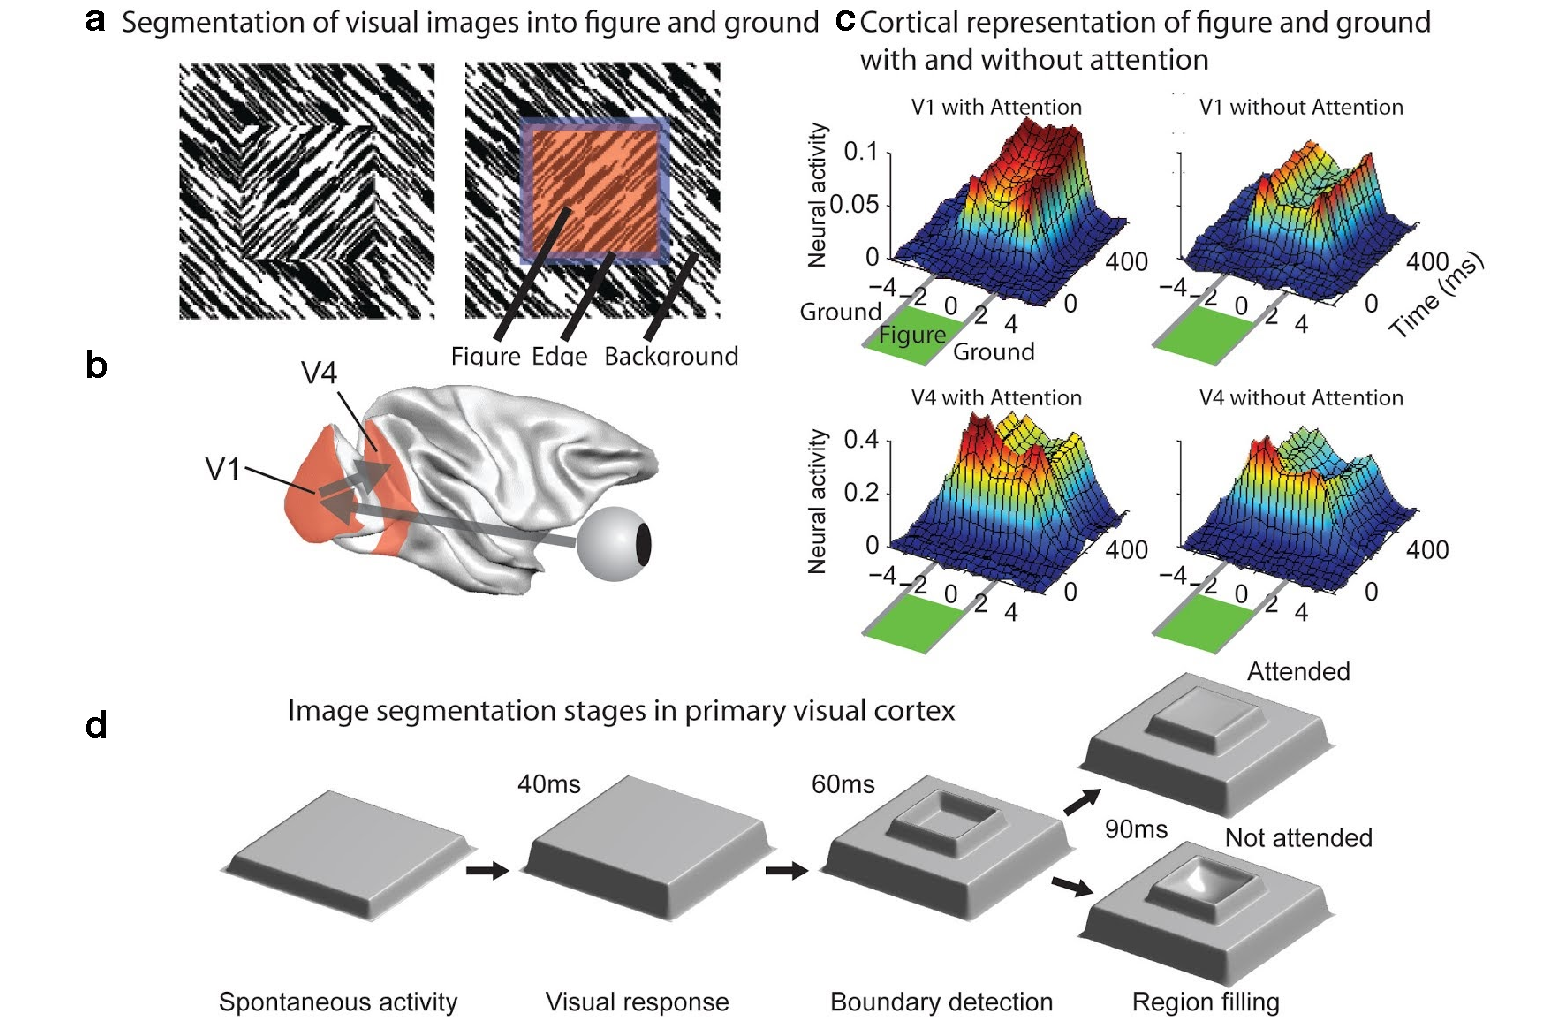
\includegraphics[width=1.\textwidth]{fig/chap4_roelfsema.pdf}
\caption[Feedback modulation of \gls{V1} activity.]{Feedback from extrastriate areas modulates \gls{V1} orientation selectivity. (a) In a task of segmenting various elements in a naturalistic context, (b) both orientation selectivity and texture selectivity, from \gls{V1} and V4 respectively, are involved. (c) The receptive field of \gls{V1} neurons changes with attention towards the figure, which is based on feedback from V4, as summarized in (d). Figures reproduced from~\cite{poort2012role}}
\label{fig_chap4_roelfsema}
\end{figure} 

Finally, \gls{V1} receives substantial and potent feedback from extrastriate cortical areas, which plays a pivotal role in shaping orientation selectivity. A salient illustration of this intricate relationship is observed in the task of figure-ground segmentation: the feedback from extrastriate areas (here, V4), allows \gls{V1} to not only to delineate the edges with precision, but also to a fully-fledged figure in meticulous details~\cite{poort2012role} (Figure~\ref{fig_chap4_roelfsema}). This feedback exhibits a broader spatial extent compared to the feedforward receptive field, adding a layer of complexity to our understanding~\cite{angelucci2006contribution}.

In predictive coding terms, such feedback mechanisms are modeled as carrying the predictions from higher-order regions to \gls{V1}. It is often implied by predictive coding these feedbacks should be modulatory only~\cite{bastos2012canonical}, in order to send prediction from higher- to lower-order areas that can suppress prediction errors produced by bottom-up input. This is however neither true~\cite{murphy1987corticofugal,wozny2011specificity, covic2011synaptic} nor required, as mixed excitatory/inhibitory influence can mediate the construction of prediction and prediction errors locally. The modular nature of this activity will be discussed further in the next chapter.

Overall, one can see how orientation selectivity in \gls{V1} is a well-defined invariant representation of low-level features of the world. As such, it serves as the perfect predictions of these features, and hence, is constrained to variance weighting, as developed in Equation~\ref{eq_pc_matrix}. While there is no clear consensus on the origin of orientation selectivity in \gls{V1}, there is no debate that the cortical circuitry is dedicated to maintain it, through a complex mix of many neural activities, that must be first recorded and then deciphered to the best of the experimenter's ability.



\section{Methods: Visual Electrophysiology and Neural Decoding}
\subsection{Recordings Tools of the Brain}

\begin{figure}[h!tbp]
\vspace{0.1cm}
\centering
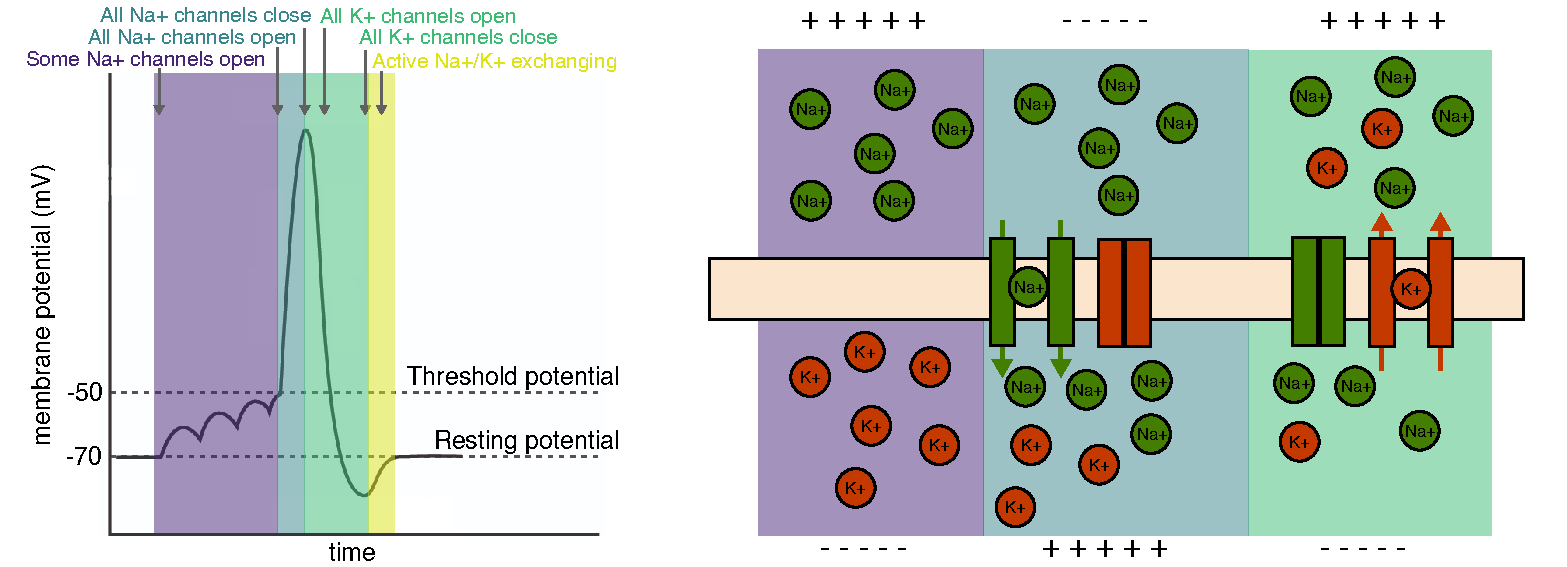
\includegraphics[width=1.\textwidth]{fig/chap4_actionpotential.pdf}
\caption[Illustration of the action potential.]{Schematic illustration of the action potential on the membrane potential (left) and its respective ionic currents (right). The final active Na+/K+ exchanging is not illustrated.}
\label{fig_chap4_actionpotential}
\end{figure} 

Neurons, as the functional units of the nervous system, communicate through sophisticated electrochemical activity, which involve using the flow of ions to generate electrical gradients~\cite{kandel2000principles}. To simplify this process, neurons effectively maintain an electrochemical gradient that puts them at an electric potential of $-70$mV with respect to their local environment. Upon binding of a neurotransmitter, channels specifically let Na$+$ ions flow through, depolarizing the neurons up to approximately $+40$mV. The neuron then activates energy-consuming K$+$ channels, re-establishing a polarized electrochemical gradient, with a slight overshooting. This change of activity propagates from the neuron's soma to its axon terminal, where it induces the fusion of synaptic vesicles through the entry of Ca$2+$ ions, resulting in the release of neurotransmitters into the synaptic cleft, which in turn can alter the conductance of the post-synaptic neuron (Figure~\ref{fig_chap4_actionpotential}). The modulation of conductance in the post-synaptic neuron is crucial as it may lead to the generation of a new action potential, thus perpetuating the chain of neural communication.

% figure recording techniques from isabelle's thesis https://www.spiedigitallibrary.org/journals/neurophotonics/volume-4/issue-03/031215/Improving-voltage-sensitive-dye-imaging--with-a-little-help/10.1117/1.NPh.4.3.031215.full?SSO=1
\begin{figure}[h!tbp]
\vspace{0.1cm}
\centering
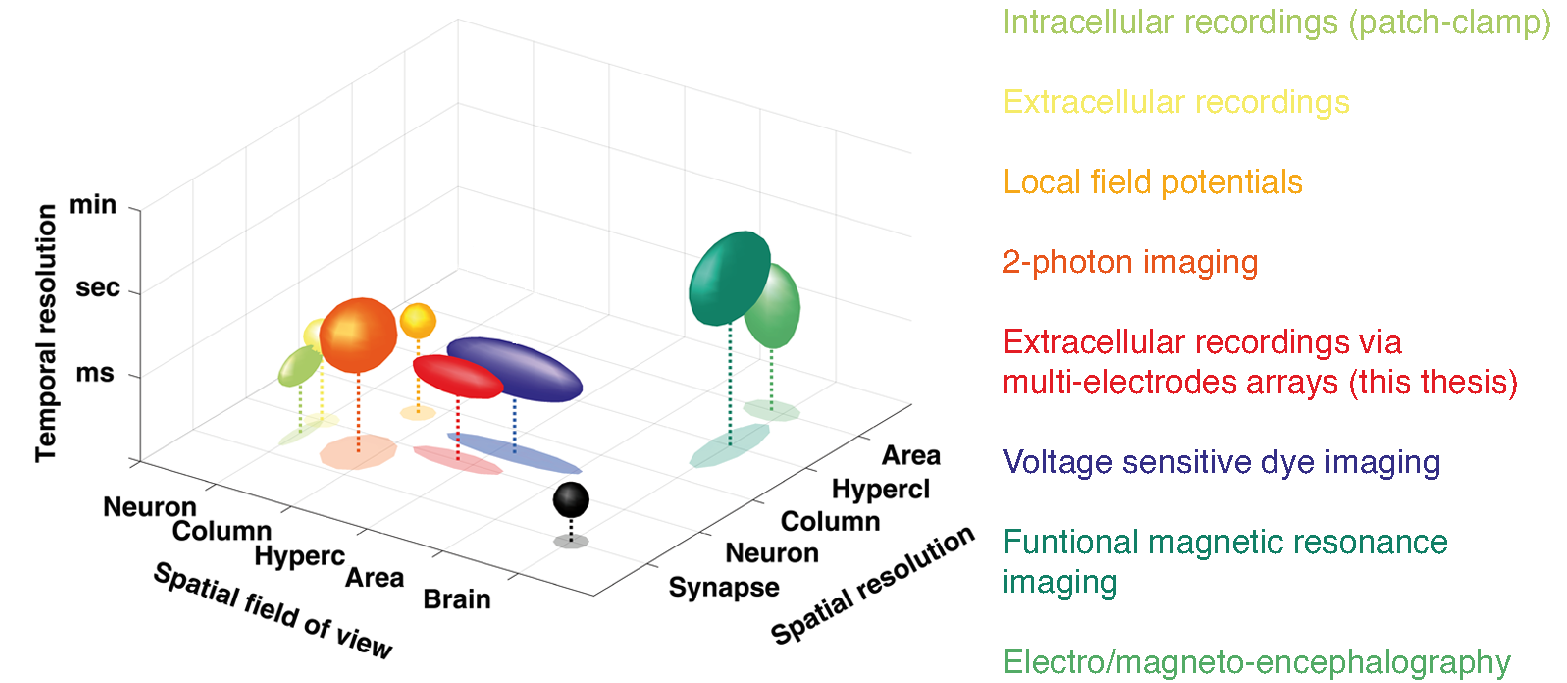
\includegraphics[width=1.\textwidth]{fig/chap4_chemla.pdf}
\caption[Methods of recording of the central nervous system.]{Spatial field of view, and spatio-temporal resolution of various methods of recordings of the nervous system, from~\cite{chemla2010voltage}.}
\label{fig_chap4_chemla}
\end{figure} 

This mechanism, (over)simplified here for clarity's sake, forms the basis of neural communication. Thus, all methods employed for recording brain activity are inherently also based on it. The lowest possible level (in terms of spatial and temporal resolution) of such recording methods consists in approaching a glass pipette with an electrode to the membrane of the neuron, then forming a seal to directly record that patch of membrane~\cite{sakmann1984patch}. This allows to record single ionic channels, which is highly effective for mapping conductance of ion to single molecules. By breaking this seal, it is possible to record the whole neuron, but also control its dynamics using current or voltage injection. Whether at the single channel or membrane level, such methods are known as "patch-clamp"~\cite{neher1992patch}, either in "current-clamp" or "voltage-clamp" mode. 

\begin{figure}[h!tbp]
\vspace{0.1cm}
\centering
\includegraphics[width=1.\textwidth]{fig/chap4_multielectrodes.pdf}
\caption[Extracellular electrodes.]{Various types of extracellular electrodes, with cortical slice of mouse visual cortex (acquired by Geneviève Cyr) for size reference. }
\label{fig_chap4_multielectrodes}
\end{figure} 

Patch-clamp techniques, while allowing to measure single neuron activity in exquisite details, cannot record from populations of neurons. Consequently, for questions related to the internal representations of certain features with an ensemble of neural activity, it is often best to measure electrical potential variations outside the neuron, which does not involve precisely putting an electrode on the neuronal membrane~\cite{buzsaki2012origin}. Rather, this method necessitates the insertion of electrodes into the brain, a procedure historically done using tungsten electrodes~\cite{hubel1959receptive, garrido2022understanding}, but nowadays predominantly achieved using multi-channel electrodes made from complex alloys~\cite{csicsvari2003massively}. This method of recording is the one used throughout this thesis (Figure~\ref{fig_chap4_multielectrodes}).

Multi-channel electrodes permit the recording of electrical activity from a multitude of neurons simultaneously, allowing extensive data collection and nuanced understanding of neural dynamics~\cite{steinmetz2018challenges,steinmetz2021neuropixels}. As of 2023, the advanced state of this technology allows for the recording of approximately one thousand neurons concurrently. Presently, we employed electrodes with lower channel counts, specifically $32$ to record neural activity. The spatial configuration of these electrodes is varied, but typically that of a linear probe, with contacts all along the vertical axis of the probe. In chapter 5, we will use a grid-like variation of that probe, which does not allow to probe for layer-specific computations, but for horizontally distributed ones instead.
Signals recorded by extracellular electrode are a mixture of activity from multiple currents and neurons near each electrode site. To assign each extracellular event to a given neuron, several algorithms exist, each performing a different (but related) version of a "spike-sorting" process. Here, Kilosort3~\cite{pachitariu2016kilosort, rossant2016spike} is used, which performs template-matching based on the extracellular events' waveforms, and has been shown to achieve state-of-the-art performance for multi-channel electrodes. Nonetheless, its output requires a (lengthy) post-processing step by the experimenter, to merge and dissociate entangled neuronal activity, which is here done with a graphical interface called "Phy"~\cite{rossant2016spike}. 

Depending on the frequency at which the signal is filtered, one can also record the local field potential from these electrodes. This constitutes a non-assigned, summed signal of all neuronal activity from neighboring units~\cite{kajikawa2011local,herreras2016local}. This technique is quite useful, because by recording the polarities of the events, one can observe the "sink" of neural activity arriving after a visual a stimulation in the layer IV of \gls{V1}, and the corresponding "source" in deeper and upper layers~\cite{schaefer2015quantification}. These sink/source terms refer to the influx of Na$2+$ ions (creating a "sink" outside the neurons) after a depolarization, and inversely for the "source". This technique is used in the present article to assign a cortical layer to the recorded neurons~\cite{ladret2023cortical}.

For the sake of a comprehensive overview, let us continue exploring the various recording tools of the brain. As far as neuron counts is concerned, increases in scale then require a change from electrodes to optical recording methods. A notable example that drives many experiments at the time of writing is calcium imaging, a technique driven by the principle that $Ca2+$ influx related to an action potential~\cite{stosiek2003vivo,friedrich2017fast}. This method enables the simultaneous recording of the activities of tens of thousands of neurons~\cite{stringer2019high}. However, its application is hampered by depth limitations, owing to the inherent constraints of optical tools in penetrating the depth of the cortex. To overcome this limitation, the exploitation of advanced physical phenomena such as two- or three-photon effects can be employed, allowing for increased depth of imaging~\cite{cheng2011simultaneous}. However, this entails a surge in the complexity of the acquisition system. The implementation of this technique also necessitates unobstructed optical access to the cortex, involving the removal of the skull for acute experiments and, in some cases, its substitution with viewing glass for chronic studies. The temporal resolution of the calcium imaging is on the scale of tens of milliseconds, which can hide single-neuron dynamics. To that end, there exists the possibility of loading the cortex with Voltage-Sensitive Dye (VSD), which loads the cortical areas with a molecule sensitive to changes in voltage~\cite{chemla2010voltage}. This technique grants superior temporal resolution~\cite{chemla2010biophysical}, allowing for detailed imaging across the entire cortical area, but most importantly, sub-action potential recordings, because it does not rely on the Ca$2+$ influx of the action potential.

At the culmination of the spectrum of recording methodologies are macroscale recordings, which encompass a range of diverse techniques, each providing unique and non-invasive insights into brain activity. Direct measurements of electrical activity can be obtained through the widely known Electroencephalography (EEG)~\cite{millett2001hans}, which measures the sink/source currents of the large cortical pyramidal neurons, offering insights into the global electrical activity of the brain~\cite{kirschstein2009source}. This is, in a way, the extra-cranial version of the recordings of Local Field Potentials described above. For finer resolution, one can rely on Magnetoencephalography, a sophisticated method that records the orthogonal magnetic field corresponding to the electrical signals generated by neural activity~\cite{hansen2010meg}. The acquisition setup is however significantly more complex, necessitating the integration of supra-conductive sensors to precisely capture the delicate magnetic fields associated with neural currents. Lastly, the mainstream method for large-brain analysis is functional Magnetic Resonance Imaging, a technique that detects the magnetic signatures of oxygen-binding molecules~\cite{worsley1995analysis,logothetis2008we}. These molecules flow into specific regions of the brain in response to neural activity to restore the local energy supply to neurons~\cite{phillips2016neurovascular}. By mapping these blood flow changes, this technique enables the indirect observation of neural activity, providing (rough) insights into the functional organization of the brain

Each of these techniques, despite their complexities and inherent limitations, contributes uniquely to our expansive view of neural activity, providing distinct insights into the dynamic interplay of neural circuits. These advanced methodologies, in conjunction with continuous advancements in neuroscientific research, are instrumental in unraveling the intricate tapestry of neuronal interactions and communications.

\subsection{Making Sense of the Recordings}
It may appear straightforward to correlate a single visual input with the quantity of spikes discharged by a single neuron and call it a code. However, this seemingly straightforward approach, formally called  "rate coding", involves the prior that the frequency of spike emissions by a neuron is presumed to signify its sensitivity to a particular stimulus. Under this paradigm, a higher spike rate is interpreted as indicative of greater neuronal responsiveness to the stimulus. As we have detailed in the introduction, this assumption stands in contrast to substantial evidence suggesting that neurons inherently strive to minimize their energy consumption as much as possible. The rate-based model, although used by Hubel and Wiesel in the original orientation-selectivity articles~\cite{hubel1959receptive, hubel1962receptive}, does not capture the full breadth of possible information strategies contained in neural recordings. 

Navigating through all the intricate mechanisms of neural coding could mandate an extra dedicated manuscript. However, the main alternative hypothesis to rate coding is temporal coding~\cite{engel1992temporal}, which posits that neurons encode information through intricate patterns in the timing of their spikes, implicating diverse aspects such as delays~\cite{grimaldi2022precise}, synchronicity, and first-spike times in the encoding process.
These multifaceted strategies all imply a different way to look at the data. This can be manageable for recordings with a low neuron count, such as an implanted electrode in a given area for an extended period of time~\cite{nougaret2023distinct}. With great sampling power comes little understandability, and with experiments with hundreds of neurons, it becomes harder to disentangle the meaning from the noise in the recordings. This is where machine learning-based approaches come in, allowing the experimenter to study its recordings with minimal prior assumptions.

\begin{figure}[h!tbp]
\vspace{0.1cm}
\centering
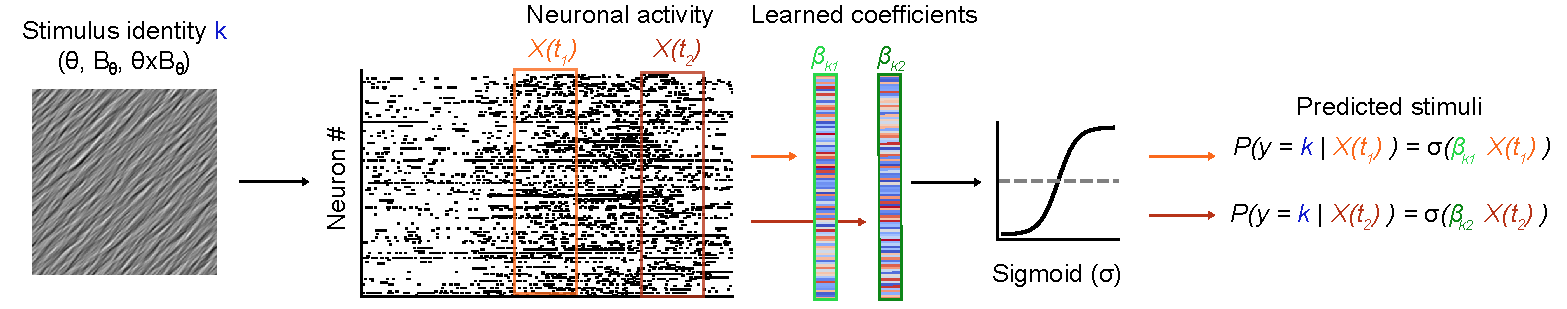
\includegraphics[width=1.\textwidth]{fig/chap4_logreg.pdf}
\caption[Illustration of logistic regression applied to neuronal decoding.]{Illustration of logistic regression applied to neuronal decoding. Additional details on the mathematical framework can be found in the chapter's article.}
\label{fig_chap4_logreg} % copy paste from previous article
\end{figure} 

As the sensory organs can essentially be seen as "encoding" the features of the world, using machine learning (or really, any non-computationally trivial) techniques to understand the neural activity is referred to as "neural decoding"~\cite{meyers2013neural,glaser2020machine}. Numerous approaches exist for neural decoding, mostly aiming to categorize neural activity into distinct types of stimuli through labelled, supervised training. The efficacy of a decoding algorithm is contingent upon its ability to discriminate between different types of neural activity; the more refined the discrimination, the more accurate the encoding of the feature to be classified within the neuron. Intuitively, this is akin to having a better separate of two conditional distributions in the neural substrate, which yields better classifier performance as the boundary between these distributions becomes better defined. For a given algorithm with optimal parametrization, improvement of the classification based on two different recordings means that features sought-after in the recordings have become more disentangled by the neurons in feature space~\cite{bishop2006pattern}. 

This forms the basis of the present article. In this research, we employ logistic regression as our neural decoder, a method praised for its simplicity, efficiency, and biological plausibility. While the implementation details are elaborated within the article, the foundational principle is depicted in the accompanying figure above. Logistic regression serves as a robust tool to unravel the complex patterns within neural datasets, allowing for the elucidation of the nuanced interactions and responses of neurons to varied stimuli.





\section{Article: "Cortical Recurrence supports Resilience to Sensory Variance in the Primary Visual Cortex"}
The following article represents a key contribution of this thesis, notably by introducing two novel neuronal responses that contribute to sensory variance encoding. Using a computational model, we validate these findings through a computational model of intracortical connectivity, which serves as the cornerstone for our argument as to how the brain processes distributions of naturalistic inputs in subsequent chapters.\\ 

Full citation is as follows: \fullcite{ladret2023cortical}
% avant d'intégrer un article dans votre thèse, consulter http://www.sherpa.ac.uk/romeo/ si vous souhaitez diffuser sur internet
\includepdfset{pagecommand=\thispagestyle{scrheadings}} % ajoute la numérotation continue des pages aux fichiers pdf importés
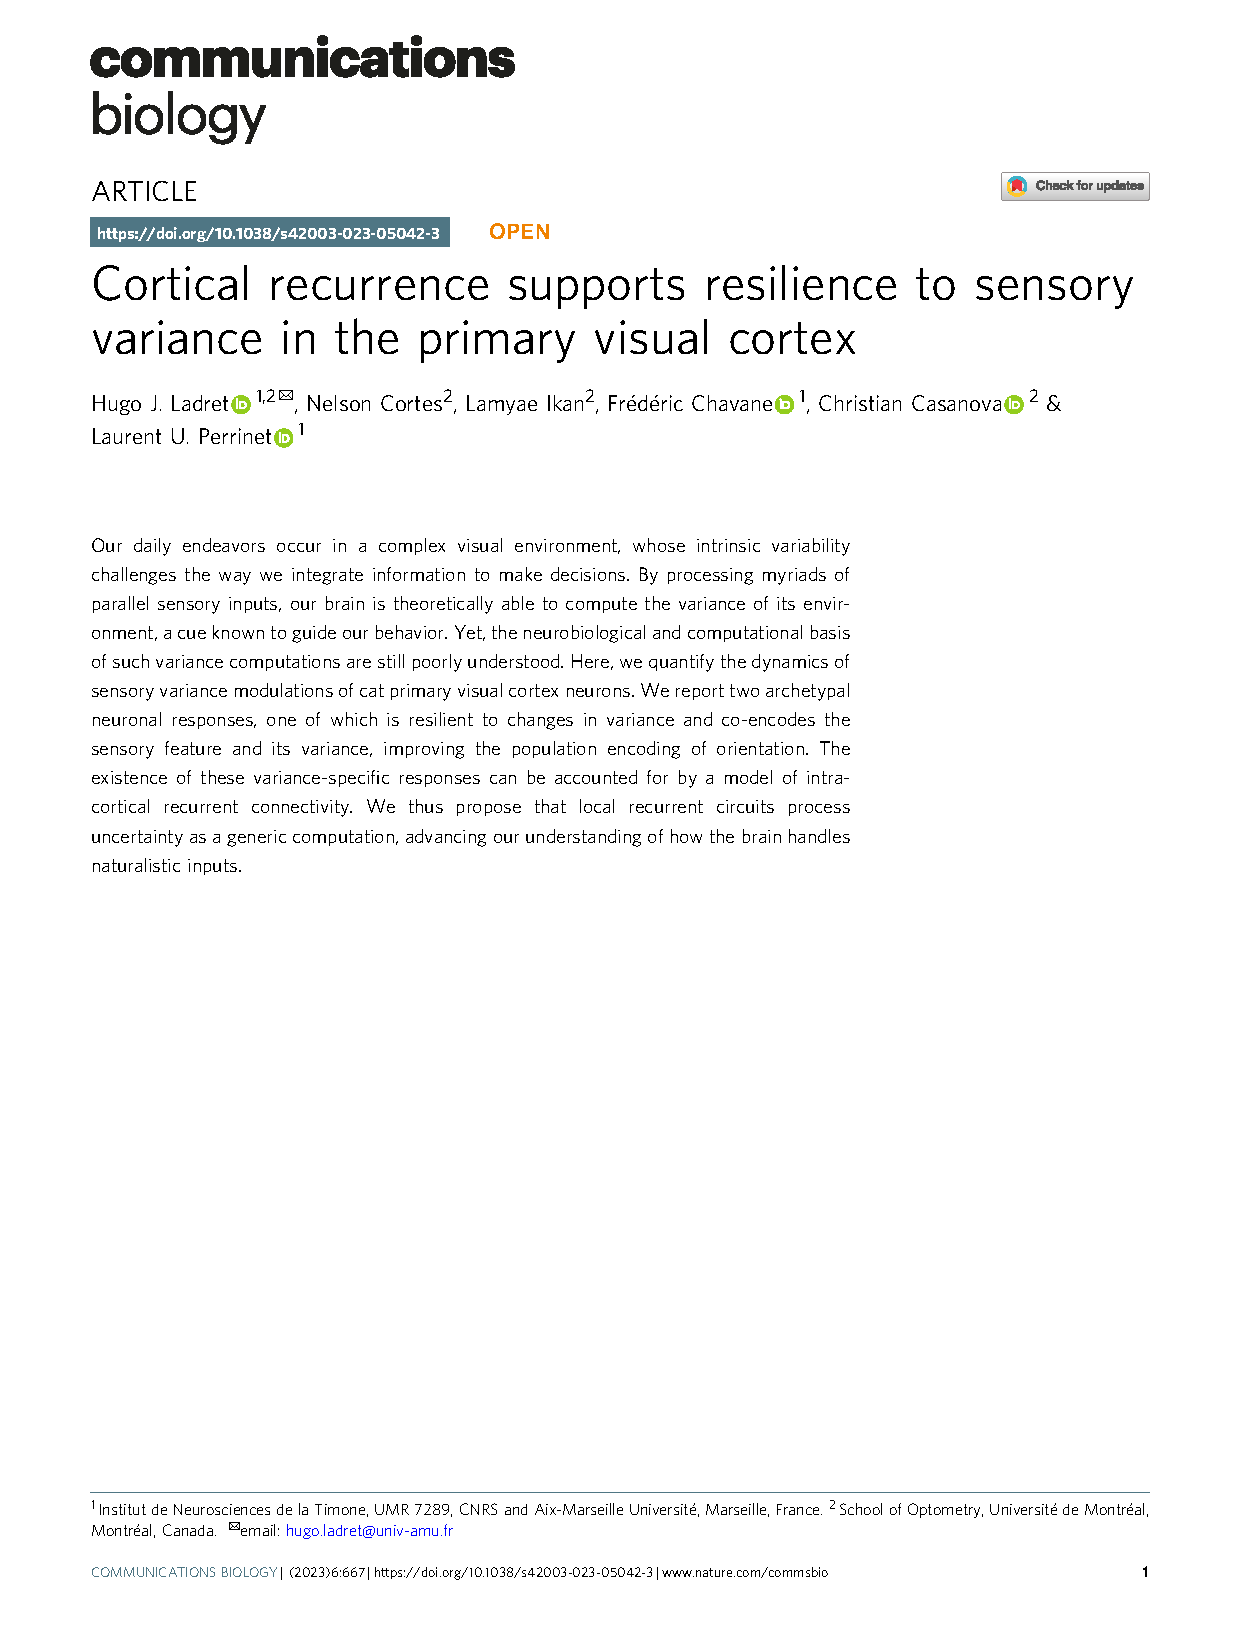
\includepdf[scale=0.82,pages=-]{papers/natcomsbio.pdf} % 'scale' ajuste la taille du pdf, vous pouvez affiner en fonction des marges




\section{Conclusion}
In this article, we have studied how the (inverse) variance of oriented inputs affects \gls{V1}. We have replicated some neural responses known in macaques\gls{V1}~\cite{goris2015origin}, extending them to complex modulations of the dynamics of single neurons and populations. Using a prior-free machine-learning approach, we have probed for neural code in the population activity, uncovering two functional types of neurons that can encode either solely the sensory feature, or jointly the sensory feature and its variance. Based on cortical layer position and on a computational approach, we propose that the processing input variance in \gls{V1} is supported by recurrent connectivity between local cortical populations.

This directly ties the present article into the predictive processing framework introduced earlier in the manuscript (Equation~\ref{eq_proba_intro}), as the experiments here essentially mean consists in manipulating the variance $\Sigma_u$ of a light pattern, in combination with its mean $g(v)$, respectively $B_\theta$ and $\theta$ in the article. While this means total access over the distribution of the input, two limitations on the predictive aspect of these recordings are missing. First, the distribution of internal priors were not controlled, for tractability's sake. This could have been done with an adaptation protocol, for example, by biasing the input over a given set of variables~\cite{damasse2018reinforcement}. Second, we did not control whether the recorded neurons were encoding prediction errors or predictions. The former is rather simple to do, by inducing a mismatch between an unexpected sequence of patterns~\cite{keller2012sensorimotor} (for example, an abrupt change of repeated orientations). The latter is more complex, as a major challenge in identifying them stems from their propensity to response like bottom-up activated neurons in various conditions~\cite{keller2018predictive}. 

Nonetheless, the present results provide an experimental validation of probabilistic processing in the brain, if not directly predictive (due to the anesthetized setup). This proves that there exists a mechanism by which the variance can weigh the activity of the \gls{V1}, essentially linking back to Equation~\ref{eq_df_derror_final}, in which the neurobiological implementation of $\Sigma_p$ and $\Sigma_u$ would be through recurrent connectivity in the brain, as predicted by the matrix form of predictive processing problems~\cite{bogacz2017tutorial} (Figure~\ref{fig_chap2_pc_matrix_graphs}). Further, the heterogeneity of recurrent connectivity, and the cross-orientation process between neurons as advanced in the final section of the article matches very well the notion that these specific interactions are competitive, inhibitory ones (Figure~\ref{fig_chap2_pc_matrix_graphs_inhibitory}).

These discoveries also have very interesting ties to canonical models of orientation selectivity, namely to complex cells. As we have mentioned in the introduction of this chapter, these cells exhibit properties that stem from a pooling of simple cells~\cite{hubel1962receptive}, but that can also stem from recurrent heavy-computations~\cite{chance1999complex}. Could it be that complex-cells are resilient cells ? A theoretical answer can be easily produced, as one could measure the phase invariance of the modelled resilient neurons in the article. An experimental answer would have required stimulating the neurons with a periodic pattern, and measuring their modulation rate~\cite{skottun1991classifying,ringach2002orientation}, which was alas not done here.

\begin{figure}[h!tbp]
\vspace{0.1cm}
\centering
\includegraphics[width=1.\textwidth]{fig/chap4_temporal_generalization.pdf}
\caption[Temporal generalization of the decoding.]{Temporal generalization of the decoding. (a) Temporal generalization matrices for decoding $\theta$ at multiple $B_\theta$. Filled white line represent onset of stimulation, and white dashed line elements where time of training and testing are identical. (b) Asymmetry of upper and lower matrices (around the diagonal). (c) Possible results from the temporal generalization process, adapted from~\cite{king2014characterizing}.}
\label{fig_chap4_temporal_generalization}
\end{figure} 

On the decoding side, our approach was based on a simplistic model of neural code, in the form of logistic regression. This was chosen for the biological plausibility of this read-out, as logistic regression essentially acting as a non-linear (sigmoidal) neuron, receiving information from the recorded spikes~\cite{berens2012fast}. Although not shown here, we also probed for a number of additional algorithms, including support vector machines, deep feedforward networks, K-nearest neighbors and random decision trees, with no accuracy benefit for these increased interpretability and complexity cost~\cite{glaser2020machine}.  
Neural decoding strategies indeed span a wide spectrum of complexity, often incorporating highly intricate methodologies that leverage non-interpretable, multifaceted aspects of neural activity. A notable advanced example is the decoding of neural activity manifolds and their correlation to behavior~\cite{chung2021neural}, a subject garnering considerable attention in modern neuroscience research. A manifold, in the realm of neural decoding, refers to a high-dimensional space (but of lower dimension than raw data) constituted by the collective activity of a group of neurons. It represents a geometric framework where each point within this space corresponds to a unique state of neural activity. Decoding the manifold implies analyzing and interpreting the intricate structures and patterns within this high-dimensional space and correlating them to specific behaviors or cognitive states. This approach to deciphering neural activity seeks to uncover the underlying structures and relationships within the neural data, potentially revealing unprecedented insights into the dynamics of neural networks and their correlations to behavioral outcomes~\cite{schneider2023learnable}. Manifold-based approach are enveloped in complexities and abstraction, but hold significant promise in advancing our understanding of the intricate interplay between neural activity and behavior.

In an earlier version of this manuscript, we placed more emphasis on the temporality of the neural code. For this, we turned to the method of temporal generalization, which consists in training the classifier on activity at a given time period, then testing it onto another one. For example, if a neural code is stable, one can train a classifier on early (post-stimulation) data, and observe good classification performance on late (post-stimulation) data. This allows to investigate whether the information carried by neuronal activity is consistent across different temporal phases following a stimulus. Further, specific shapes of the temporal generalization matrix can be (theoretically) tied to specific patterns of propagation of activity between neurons (Figure~\ref{fig_chap4_temporal_generalization}). In the present case, this was used to find a series of non-reversible neural codes, i.e. computations that do not generalize in both time directions which is a hallmark of a sequential, iterative computation~\cite{king2014characterizing}. More specifically, low variance stimulation contained maximally informative neural code early in the onset of the post-stimulation activity, which disappeared afterward. For high variance stimulation, the information was contained in later timestamps, which ultimately informs us on a time-dependent neural code (unsurprising, given single neurons dynamics shown in the article).

\begin{figure}[h!tbp]
\vspace{0.1cm}
\centering
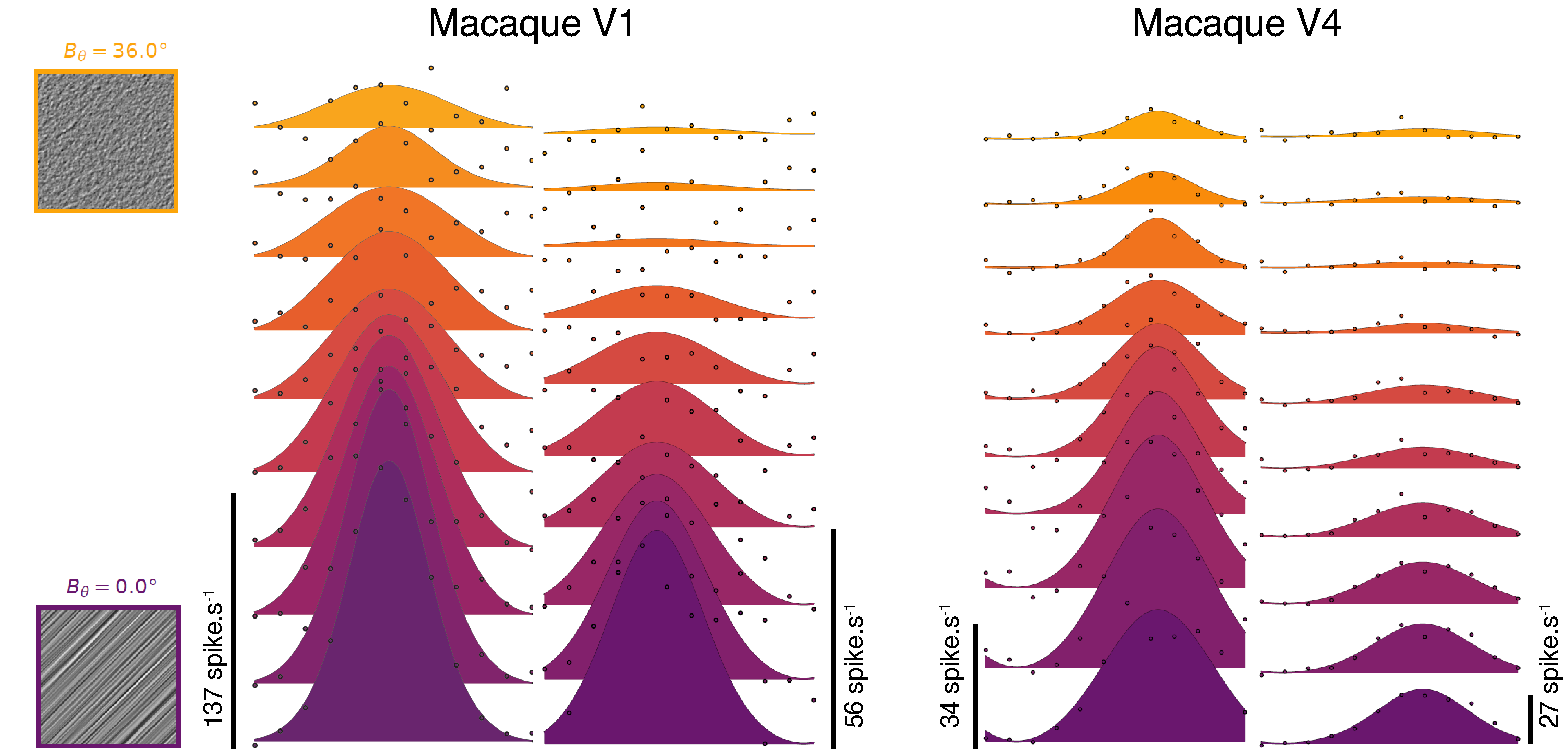
\includegraphics[width=1.\textwidth]{fig/chap4_utah_array.pdf}
\caption[Orientation variance modulations in macaques.]{Orientation variance modulations in macaque \gls{V1} and V4. Stimulation protocol is similar to the one presented in this chapter's article. These results will be further elaborated upon in chapter 5.}
\label{fig_chap4_utah_array} 
\end{figure} 

After having shown in this article a laminar (i.e., vertical) organization of variance computations, we turned to a new type of extracellular electrodes to extend those results. As interactions between neurons with different preferred orientation requires sampling of the orientation map, a horizontal probe is better suited to this task. As such, our results we replicated in awake macaque in Pieter Roelfsema's laboratory, using Utah arrays (Figure~\ref{fig_chap4_utah_array}), which are matrices of electrodes, consisting of $128$ recording sites in a 8x8 grid. Using the exact same type of stimulations (MotionClouds, rigit drift orthogonal to median orientation), we replicated similar neuronal behavior from anesthetized cats to awake primates, but also to extend our results into extrastriate areas, namely in V4. Interestingly, this not only holds for the single isolated neurons as shown in Figure~\ref{fig_chap4_utah_array}, but also for the response of neurons that are anatomically grouped. The specific advantages of this method of sampling are showcased in chapter 5, in which we infer functional connectivity directly into this data.


